\section{Introduction}
% WHERE: application in HRI
Robots deployed to unstructured environments demand a delicate balance between adaptability and motion consistency. While the robot must efficiently accomplish its designated tasks, it is equally essential to ensure the safety of its movements by avoiding collisions at all times. This becomes especially relevant in physical human-robot collaboration \parencite{ajoudani2018progress}.

% Fast control -> closed form DS
Central to controlling a robot is obtaining the desired velocity that guides it toward the goal. In complex and dynamic environments, velocities must be updated in real time based on incoming information about the surroundings. This necessitates algorithms that are easy to parameterize and fast to evaluate. 
This can be achieved by a closed-form control law, which eliminates the need for constant replanning. In this context, Dynamical Systems (DS) have been used to represent the desired motion of the system, which is approximated through an appropriate controller. DS can be designed with well-known tools from control theory to provide stability and convergence guarantees for navigation in dynamic environments.

% Compliance [Stay Reactive]
Human muscles can quickly adapt to external forces; the flexible design of our bodies allows us to deploy variable stiffness to absorb shock and impacts. 
Conversely, most robotic systems are made of stiff metallic or plastic material. 
As a result, physical interaction with the environment leads to abrupt transfer of energy and potentially damage to the system or its environment. However, modern robotic platforms often have force and torque sensing capabilities, which allow for the precise control of the effort exerted by the robot.
Yet, this results in a control problem with multiple constraints: the robot should reach the specified position while maintaining a desired velocity and remaining compliant with interaction forces. This control problem, of balancing position, velocity, and force constraints can be addressed using \textit{impedance controllers} \parencite{takegaki1981new, hogan1985impedance}.

% Ensure Obstacle Avoidance
Obstacle avoidance is a fundamental task of motion control, and reactive approaches exist that can handle dynamic and complex environments \parencite{huber2022avoiding}. 
However, incorporating obstacle avoidance together with co requires careful design. The controller should remain compliant in free space and follow the desired motion. When approximating the obstacle's surface, such as glass on the table, the controller must remain stiff and not accidentally tip over the glass, yet when interacting with an operator it is safer to be compliant (Fig.~\ref{fig:table_avoidance_with_obstacle}). 
Such a design requires a variable impedance controller, which weights different goals, such as following the desired dynamic versus remaining compliant to external forces \parencite{kronander2015passive}. 

\begin{figure}
\centerline{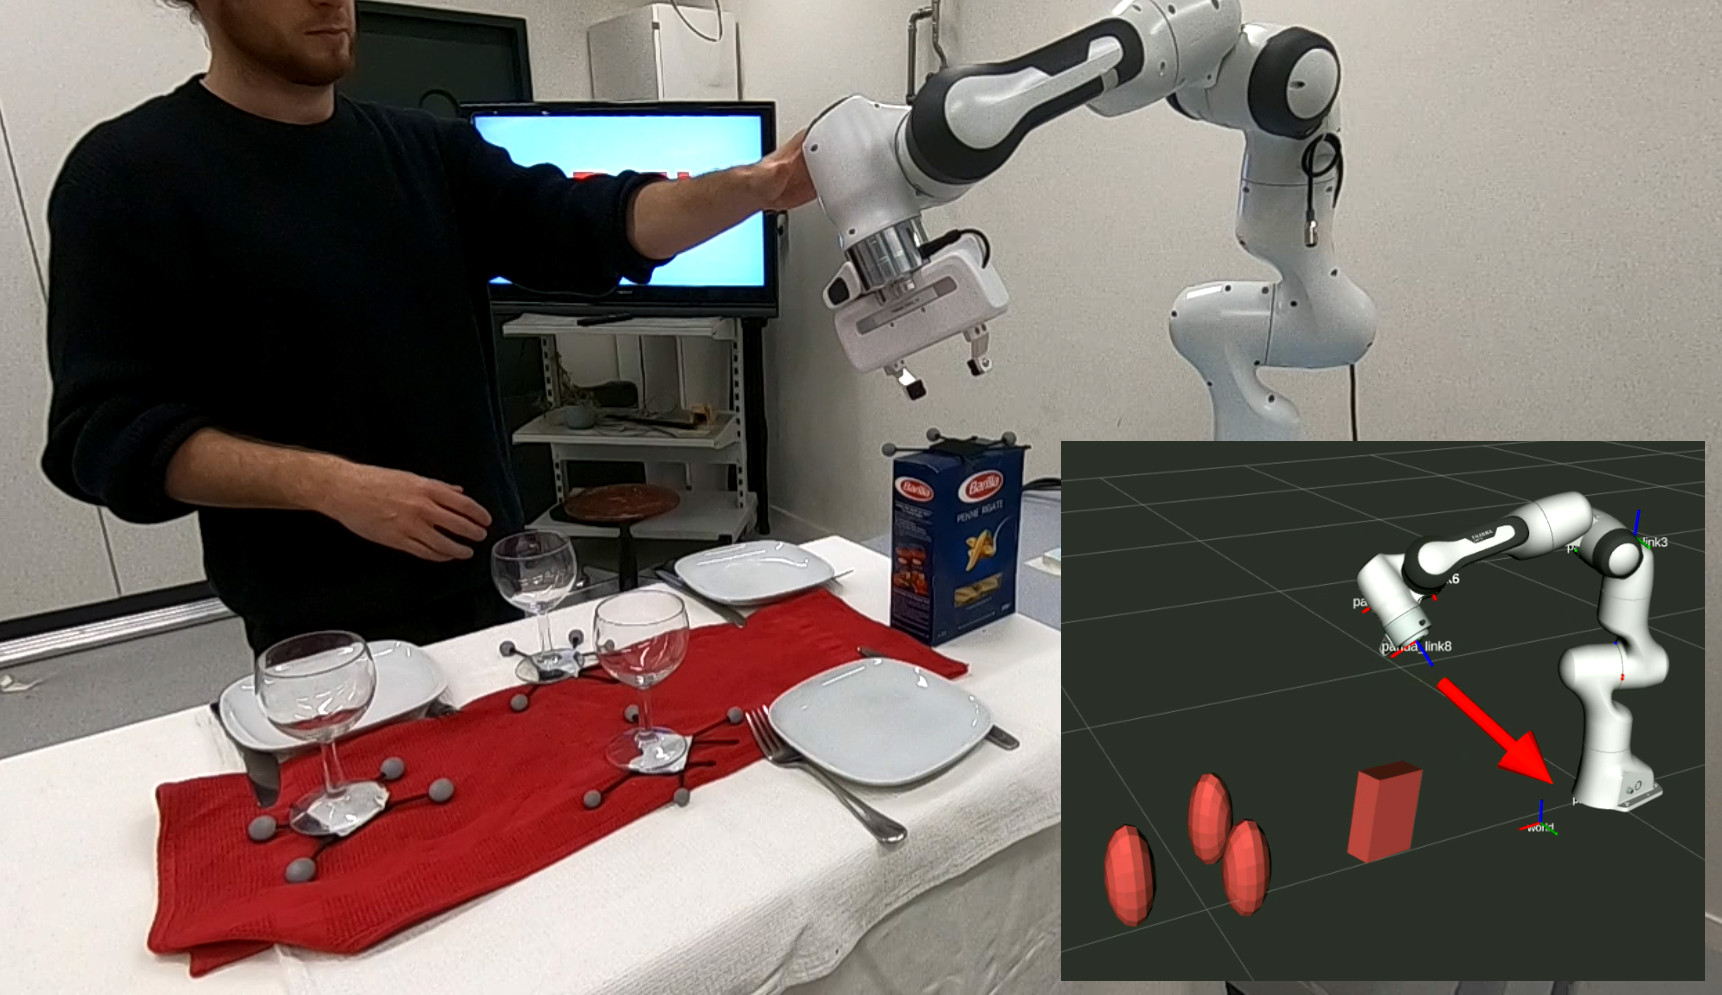
\includegraphics[width=0.5\textwidth]{figures/robot_arm_table_avoidance}}
\caption{
The proposed passive obstacle-aware controller lets the robot absorb external disturbances while ensuring collision avoidance. 
While tipping over the closed pasta box on this dinner table setup might be acceptable. Yet, the delicate wine glasses demand careful handling to prevent breakage.
}
\label{fig:table_avoidance_with_obstacle}
\end{figure}

This work incorporates dynamic obstacle avoidance using DS and variable impedance control, enhancing robotic movements' adaptability, reactivity, and safety. It allows the robot to navigate complex environments while proactively avoiding collisions and adeptly rejecting disturbances. We evaluate the performance of our approach through extensive simulations and practical implementation on a 7DoF robot arm, achieving robust and safe robot control in real-world scenarios.

\subsection{Related Work}

\subsubsection{Impedance Control}
Impedance control, a powerful feedback algorithm, effectively applies Cartesian impedance to nonlinear manipulators' end-points \parencite{takegaki1981new, hogan1985impedance}. The controller replaces the computationally intensive \textit{inverse kinematics} with the more straightforward \textit{forward kinematics}. Impedance control establishes a dynamic relationship between desired position, velocity, and force, offering a holistic control framework.
Initially, impedance controllers employed constant stiffness, but researchers have explored various dynamic control parameter approaches to enhance adaptability in complex environments \parencite{vanderborght2013variable, abu2020variable}. However, introducing dynamic parameters into the control framework requires taking special care of the system's stability.
Furthermore, admittance control is designed to adapt to external forces, while remaining stable contact \parencite{glosser1994implementation}. Admittance control can be interpreted as a special type of impedance control.

% Passivity with increased precision
Passive velocity controllers use a state-dependent velocity, which is converted into a control force through a damping control law. Since the controllers have variable damping parameters, stability can be guaranteed using storage tanks inspired by a virtual flywheel \parencite{li1999passive}. 
Furthermore, complex control parameters can be learned from human demonstrations. By continuously adapting the parameters, the controller can be observed to improve its tracking performance in direct human-robot collaboration tasks \parencite{gribovskaya2011motion}.
However, high compliance often results in decreased motion following. Yet, carefully designing the damping matrix, which increases stiffness in the direction of motion, but remains compliant otherwise, results in improved convergence \parencite{kronander2015passive}. 
Combining impedance controllers with admittance controllers can be used to increase accuracy in cooperative control
\parencite{fujiki2022series}.
However, these controllers' adaptations focus on improving movement accuracy rather than actively rejecting disturbances.

% Stable interaction controller
Impedance controllers play an important role in interaction tasks, as in these situations, the robot is subjected to forces that are hard to predict precisely. However, they must be actively managed to ensure stable contact without damage occurring. In these situations, passive controllers using storage tanks based on the system's energy allow to limit contact force \parencite{kishi2003passive}.
A general framework can be used to ensure that position-, torque-, and impedance controllers exhibit passivity during interaction tasks. This is achieved by interpreting the torque feedback as the shaping of the motor inertia. It allows the use of flexible robot arms for complex interaction tasks, such as insertion or wiping \parencite{albu2007unified}. 
By sensing the interaction force and actively adapting the trajectory based on the physical interaction force and the virtual repulsive force from the obstacle. This can be used for obstacle-aware motion generation \parencite{haddadin2010real}.
% Telemanipulation
Teleoperated systems of robot arms come with control delays and require a closed-loop controller of the robot that can adapt autonomously, ensuring stable and reliable performance. Passive controllers present themselves perfectly for such a task  \parencite{stramigioli2005sampled}. This method addresses the intricate dynamics of interactive systems, ensuring stable and reliable performance.
A similar approach involves slowly updating the desired position while incorporating a spring-damper model through an impedance controller, enabling seamless interaction with the teleoperated robotic system \parencite{lee2010passive}.
However, these models require human input for active collision avoidance.

% Energy tanks 
Many impedance controllers with time-varying control rely on energy tanks to ensure stability. This is a virtual state of the system, which is filled or emptied depending on the controller command. Limiting the energy tank to a maximum value ensures the system's stability  \parencite{ferraguti2013tank}. However, when this limit is reached, the controller is constrained and interferes with the controller's optimal functioning. This can result in the controller not achieving a main functionality, such as collision avoidance.
Alternatively, the impedance controller variables can be constrained by adapting the damping and stiffness, as well as their rate of change based on a Lyapunov function \cite{kronander2016stability}.

\subsubsection{Obstacle Avoidance}
% AFP / Obstacle avoidance / Motion Control
In dynamic environments, obstacle avoidance has to be quickly evaluated to ensure safe robot navigation. Repulsive force fields pointing away from obstacles can be used to create a collision-free motion \parencite{khatib1987unified}. 
However, these artificial potential fields are susceptible to local minima, which led to the introduction of navigation functions. A global function that combines the repulsive force fields while ensuring a global minimum and the goal \parencite{koditschek1990robot}. However, such functions depend on the distribution of the obstacles and are hard to adapt to dynamic environments and high dimensional spaces \parencite{loizou2022mobile}.


% \cite{brock2002task}, % Corresponding conference 
Passive controllers can also be used to track the desired motion of the artificial potential field while compensating for Coriolis and centrifugal forces \parencite{duindam2004passive}. 
Nonetheless, these methods lack the guarantee of disturbance repulsion around obstacles, which is addressed by the integration of circular fields, which rotates the robot's path around the obstacles \parencite{singh1996real}. 
This allows force-controlled navigation in cluttered environments, yielding convergence for simple obstacles \parencite{haddadin2011dynamic}. 
Conversely, repulsive fields can be combined with elastic, global planning \parencite{brock2002elastic} for improved convergence. This allowed adding a repulsive force from the obstacle, ensuring collision avoidance \parencite{tulbure2020closing}. 
However, methods based on artificial potential fields are prone to local minima in space around cluttered environments.

% Geometric Methods for Obstacle Avoidance / Force Control
Traditional tracking controllers often require complex linearization or simplification methods. However, a class of geometric tracking controllers enables exact control of nonlinear mechanical systems with low computational cost \parencite{udwadia2003new}. By reformulating control problems as a specific class of optimal controllers, this approach facilitates the derivation of standard control problems in robotics \parencite{peters2008unifying}. As a result, many geometric controllers directly output a control force, and hence do not rely on an additional (impedance) controller.
Integrating local Riemannian Motion Policies (RMP) has led to globally stable force-controlled motion \parencite{cheng2020rmp}. Moreover, advancements in position-dependent Riemannian metrics allow for improved task design using RMP and reactive force control under constraints \parencite{bylard2021composable}.
Geometric fabrics have emerged as a valuable mathematical tool for shaping a robot's nominal behavior while capturing essential constraints like obstacle avoidance, joint limits, and redundancy resolution \parencite{xie2020geometric}. Combining Finsler geometry and geometric fabrics has further enhanced path consistency \parencite{ratliff2021generalized}.
Integrating geometric fabric methods into classical mechanical systems has enabled various physical behaviors, notably exemplified in multi-obstacle avoidance for a 7DoF robot arm \parencite{van2022geometric}. Despite these significant achievements, the parametrization of geometric methods and their application to general systems remains challenging and hinders their wide acceptance.

% Dynamical system based avoidance + control
Harmonic potential functions can ensure the absence of local minima in free space \parencite{connolly1997harmonic}. In previous work, we combined harmonic potential functions with the dynamical system framework to obtain reactive, local minima-free motion \parencite{huber2019avoidance, huber2023avoidance}. It allows for generating a desired velocity based on the robot's position in real-time.
For implementation on a torque-controlled robot arm, we utilized a passive controller that closely adheres to the desired velocity \parencite{kronander2015passive}. However, one of the limitations of the passive controller is its inability to  account for the physical surroundings. This makes the robot susceptible to disturbances close to obstacles, potentially leading to collisions.

Although DS passive-controlled robots work well in interactive scenarios, they cannot ensure they navigate through an obstacle environment collision-free. For example, they often give in when being pushed toward an obstacle. This work presents a method to address this problem by modifying the passive control law design, making the controller aware of its environment.

\subsection{Contribution}
We introduce a passive controller that incorporates into the feedback control loop as visualized in Figure~\ref{fig:control_scheme_passive}. 
In this work, we make the following contributions:
\begin{itemize}
\item The design of the obstacle-aware passive controller
(Section~\ref{sec:obstacle_aware_passivity})
\item A passivity guarantee (without the need for a storage tank) which applies to general damping controllers (Theorem~\ref{theorem:passivity})
\item A collision avoidance analysis which provides insight into the path consistency around obstacles (Section~\ref{sec:collision_avoidance})
\item Discrete-time analysis to enable control parameter design which ensures stability (Section~\ref{sec:discrete_time_behavior})
\item Implementation and testing on 7DoF robot arm (Section~\ref{sec:evaluation})
\end{itemize}


\begin{figure}[thb]
  \center
  \includesvg[width=1.0\columnwidth]{figures/control_scheme_passive.svg}
\caption{The desired velocity $\vect f^b(\vecs \xi)$ can result from a learned velocity field or pointing towards a desired attractor $\vecs \xi^a$. The desired velocity is used to evaluate the obstacle avoidance velocity $\vect f(\vecs \xi)$, which is fed into the force controller to obtain the control force $\vect \tau_c$. In order to achieve collision avoidance, the distance function $\Gamma_o(\vecs \xi)$, the normal direction $\vect n_o(\vecs \xi)$, and the reference direction $\vect r_o(\vecs \xi)$ are evaluated for each obstacle $o = 1 .. N^\mathrm{{obs}}$.}
\label{fig:control_scheme_passive}
\end{figure}
